% =============================================================================
% Slide deck -- ambient-electron exchange thruster, for an EP-engineer audience
% Build: pdflatex slides.tex (twice). Assets shared with ../main.tex (../figs).
% Organization: objections first (return current, F/P), then measurements,
% then credibility + honest limits. Assertion-as-title style.
% =============================================================================
\documentclass[10pt,aspectratio=169]{beamer}
\usetheme{default}
\usecolortheme{seahorse}
\setbeamertemplate{navigation symbols}{}
\setbeamertemplate{footline}[frame number]
\setbeamercolor{frametitle}{fg=blue!30!black}
\setbeamerfont{frametitle}{series=\bfseries,size=\large}
\usepackage{booktabs,tikz,graphicx}
\graphicspath{{../figs/}}
\newcommand{\srcnote}[1]{\vfill{\tiny\color{gray}#1}}

\title{Propellantless Drag Compensation by Ambient-Electron Exchange}
\subtitle{Ion-thruster efficiency at nanonewton scale, zero propellant\\
{\small three gated PIC operating points -- pre-registered predictions -- a measured thrust--power frontier}}
\author{R.~S.~C.}
\date{August 2026}

\begin{document}

% 1 ---------------------------------------------------------------------------
\begin{frame}
  \titlepage
\end{frame}

% 2 ---------------------------------------------------------------------------
\begin{frame}{The nN/mW corner of the thrust--power plane is empty}
  \begin{columns}
    \column{0.62\textwidth}
      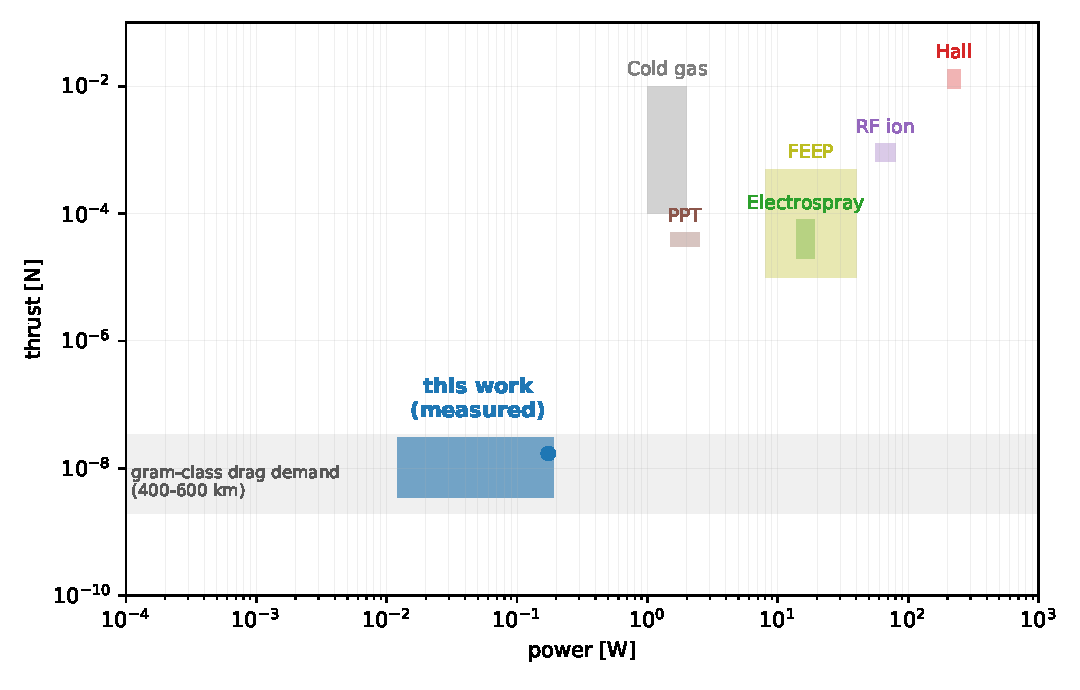
\includegraphics[width=\linewidth]{fp_plane.pdf}
    \column{0.36\textwidth}
      \begin{itemize}\small
        \item Gram-class spacecraft at 400--600\,km need \textbf{2--30\,nN
              continuous} from a \textbf{mW-class} budget.
        \item Smallest flight EP (FEEP/electrospray): 5--30\,\textmu N,
              $\ge$8\,W, kg-class systems -- $10^2$--$10^3\times$ above the
              demand on every axis.
        \item Tanked systems don't shrink: tank + feed + valves + PPU
              $\approx$ 0.3--1\,kg \emph{dry}, at any propellant load.
      \end{itemize}
  \end{columns}
  \srcnote{Incumbent ranges: NASA SoA Small Spacecraft Technology 2026;
  manufacturer datasheets (see paper Table 2).}
\end{frame}

% 3 ---------------------------------------------------------------------------
\begin{frame}{You already fly this device --- as a neutralizer}
  \begin{columns}
    \column{0.52\textwidth}
      \centering
      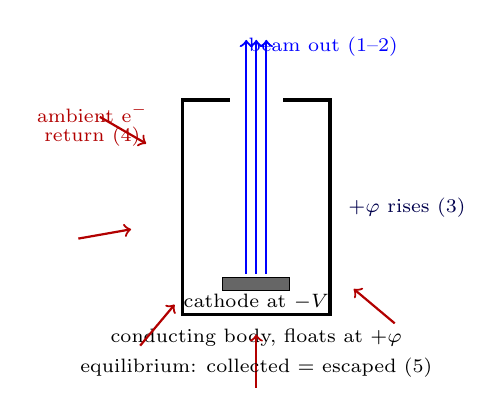
\begin{tikzpicture}[scale=0.85, every node/.style={font=\scriptsize}]
        % body
        \draw[very thick] (0,0) rectangle (2.2,3.2);
        \draw[very thick,white,line width=3pt] (0.7,3.2) -- (1.5,3.2);
        \draw[very thick] (0.7,3.2) -- (0.7,3.2);
        \node at (1.1,-0.35) {conducting body, floats at $+\varphi$};
        % cathode
        \draw[fill=black!60] (0.6,0.35) rectangle (1.6,0.55);
        \node at (1.1,0.18) {cathode at $-V$};
        % beam
        \foreach \x in {0.95,1.1,1.25}
          \draw[->,thick,blue] (\x,0.6) -- (\x,4.1);
        \node[blue] at (2.1,4.0) {beam out (1--2)};
        % aperture marks
        \draw[very thick] (0,3.2) -- (0.7,3.2);
        \draw[very thick] (1.5,3.2) -- (2.2,3.2);
        % returning electrons
        \foreach \a in {150,190,230,270,320}
          \draw[<-,thick,red!70!black]
            ({1.1+1.9*cos(\a)},{1.6+1.9*sin(\a)}) --
            ({1.1+2.7*cos(\a)},{1.6+2.7*sin(\a)});
        \node[red!70!black] at (-1.35,3.0) {ambient e$^-$};
        \node[red!70!black] at (-1.35,2.65) {return (4)};
        \node at (3.35,1.6) {\color{blue!30!black}$+\varphi$ rises (3)};
        \node at (1.1,-0.8) {equilibrium: collected = escaped (5)};
      \end{tikzpicture}
    \column{0.46\textwidth}
      \begin{enumerate}\small
        \item Supply holds cathode at $-V$ relative to the body.
        \item Electrons accelerate out through one aperture
              (KE $\approx 0.81\,e(V-\varphi)$, measured).
        \item Body charges positive.
        \item Ionosphere returns the current to the skin.
        \item Balance closes: \textbf{the ionosphere is propellant tank
              and neutralizer.}
      \end{enumerate}
      \vspace{1ex}
      \small Hardware: an HV supply, a cold gun, a hole.
      \textbf{Every ion/Hall thruster already carries the gun} -- run alone,
      it is this thruster (retrofit path after propellant exhaustion).
  \end{columns}
\end{frame}

% 4 ---------------------------------------------------------------------------
\begin{frame}{``The current comes back --- doesn't the momentum cancel?'' We measured it: no.}
  \begin{columns}
    \column{0.55\textwidth}
      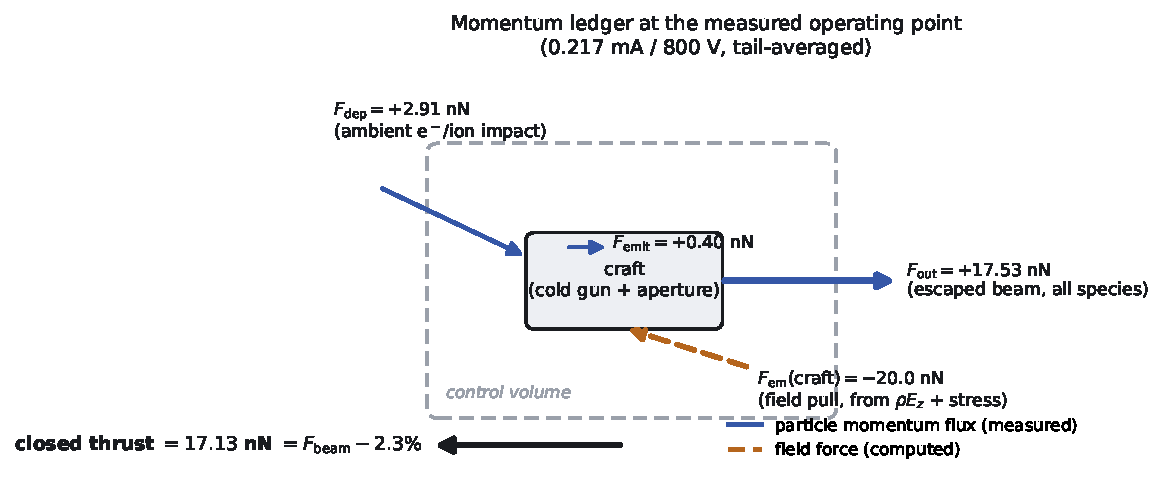
\includegraphics[width=\linewidth]{ledger_diagram.pdf}
    \column{0.43\textwidth}
      \textbf{Full-return null test} (predecessor implementation): body
      pinned above beam energy, escape $= 0$\%.\\[0.5ex]
      \small impact channel alone: $-12.1$\,nN\\
      closed thrust: $-0.39\,\text{nN} \approx 0$ \hfill $\checkmark$\\[1ex]
      \normalsize\textbf{At the operating points} (this campaign, gated
      per run):\\[0.5ex]
      \small all-species impact momentum vs beam thrust:\\
      \textbf{1.0\%} at 300\,V \quad (0.30 vs 30.13\,nN)\\
      \textbf{8.8\%} at 100\,V\\[1ex]
      Physics ceiling: collected e$^-$ arrive isotropically at
      $\sim e\varphi$ (36\,eV) vs 210\,eV directed exhaust --- even fully
      anti-directed arrival cancels $\le\sqrt{\varphi/\mathrm{KE}}
      \approx 41\%$.
  \end{columns}
\end{frame}

% 5 ---------------------------------------------------------------------------
\begin{frame}{Our $F/P$ is 200$\times$ below your Hall thruster --- by design, not by failure}
  \centering
  \begin{tabular}{lccc}
    \toprule
     & \textbf{this work} & electrospray / FEEP & Hall \\
    \midrule
    energy conversion $\eta_{\mathrm{jet}}$ & \textbf{68--73\,\%} & 28--45\,\% & $\approx$31--44\,\% \\
    thrust per watt & 0.16--0.28\,\textmu N/W & $\sim$5\,\textmu N/W & $\sim$50\,\textmu N/W \\
    \bottomrule
  \end{tabular}
  \vspace{2ex}
  \begin{itemize}\small
    \item Both rows are true at once \emph{because the exhaust is electrons}:
          superb energy-to-jet conversion at tiny momentum per watt.
    \item The $F/P$ penalty is \textbf{invisible at nN (mW)}, noticeable at
          \textmu N ($\sim$10\,W for CubeSat drag -- disqualifying), decisive
          at mN.
    \item The handoff is part of the claim: \textbf{this device below
          $\sim$0.1\,\textmu N, electrospray at \textmu N, ion/Hall at mN.}
          We are your complement, not your competitor.
  \end{itemize}
  \srcnote{$\eta$ sources: Busek BET-MAX datasheet; Krejci et al.\ 2019 (IFM);
  computed from BHT-200 figures. See paper Table 2 sourcing notes.}
\end{frame}

% 6 ---------------------------------------------------------------------------
\begin{frame}{Spacecraft charging is the operating principle, not a failure mode}
  \begin{columns}
    \column{0.5\textwidth}
      \begin{itemize}\small
        \item The float $\varphi$ is the state variable: it rises until the
              ionosphere returns exactly the escaped current.
        \item Measured floats across the hardware range:
              \textbf{$+5.4$ / $+17.0$ / $+36.3$\,V} at 100/200/300\,V.
        \item Gated benign ($\varphi \le 50$\,V) on every run; a runaway-%
              charging (choke) detector aborts any run the ionosphere cannot
              neutralize.
        \item The float robs the beam: accelerating potential is always
              $V - \varphi$ (charging tax: 5\% at 100\,V, 12\% at 300\,V).
      \end{itemize}
    \column{0.48\textwidth}
      \centering
      \begin{tabular}{lccc}
        \toprule
        $V$ [V] & 100 & 200 & 300 \\
        \midrule
        $\varphi$ [V] & $+5.4$ & $+17.0$ & $+36.3$ \\
        escape & 96.1\% & 98.4\% & 99.0\% \\
        balance & 1.5\% & 3.2\% & 3.5\% \\
        \bottomrule
      \end{tabular}
  \end{columns}
\end{frame}

% 7 ---------------------------------------------------------------------------
\begin{frame}{The frontier is measured, not projected}
  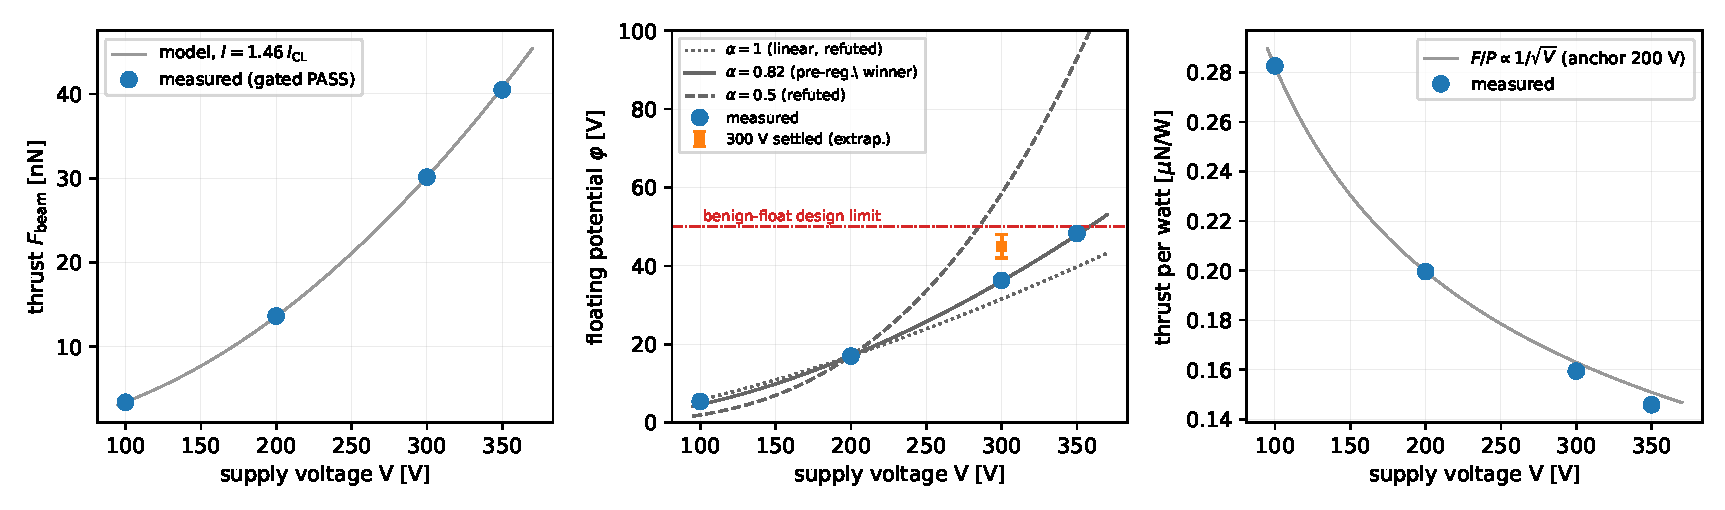
\includegraphics[width=\linewidth]{frontier.pdf}
  \begin{itemize}\small
    \item Three production runs across the full 100--300\,V hardware range;
          \textbf{all pre-registered acceptance gates PASS} on each.
    \item $F/P \propto 1/\sqrt{V}$ confirmed within 2.5\,\%; thrust landed
          $<$1\,\% from predictions \emph{recorded in the repository before
          the runs completed}.
  \end{itemize}
\end{frame}

% 8 ---------------------------------------------------------------------------
\begin{frame}{The collection law was decided by experiment}
  \begin{columns}
    \column{0.5\textwidth}
      \small
      Collected current: $I = \beta A\, j_{\mathrm{the}}\,(1+\chi)^{\alpha}$,
      \ $\chi = e\varphi/kT_e$.\\[1ex]
      Three exponents in the lineage, all agreeing at the 200\,V anchor,
      diverging at 300\,V ($\chi \approx 320$). Predictions recorded before
      the run:
      \begin{center}
      \begin{tabular}{lcc}
        \toprule
        law & predicted $\varphi$(300\,V) & verdict \\
        \midrule
        $\alpha = 1$ (linear) & 31\,V & \textcolor{red}{refuted} \\
        $\alpha = 0.82$ & 36\,V & \textcolor{green!50!black}{\textbf{survives}} \\
        $\alpha = 0.5$ & 90\,V & \textcolor{red}{refuted} \\
        \midrule
        \textbf{measured} & \textbf{36.3\,V} & \\
        \bottomrule
      \end{tabular}
      \end{center}
    \column{0.48\textwidth}
      \small
      \begin{itemize}
        \item Fit across all three points: $\alpha = 0.85$--0.89.
        \item Pre-registered caveat honored: the 300\,V float was still
              relaxing (settled band $\approx$42--48\,V, inside the 50\,V
              limit) -- carried as uncertainty, not hidden.
        \item This is the physics that sets the operating point -- and it
              collapses the throttle policy into\ldots\ (next slide)
      \end{itemize}
  \end{columns}
\end{frame}

% 9 ---------------------------------------------------------------------------
\begin{frame}{The optimal controller is two lines on the spacecraft's own float}
  \begin{block}{The flight rule (measured constants, no ionosphere model, no lookup table)}
    \centering
    \begin{tabular}{l}
      1.\quad $V \approx 3.1\,\varphi$ \hfill (servo the supply to the measured float)\\[0.4ex]
      2.\quad $I = F_{\mathrm{req}} / \big(3.27\sqrt{0.81\,(V-\varphi)}\big)$
        \hfill (current from thrust demand)\\[0.4ex]
      \quad\ \ guards: $I \le 1.46\,I_{\mathrm{CL}}(V)$;\quad
        $\varphi \le 50$\,V;\quad infeasible $\Rightarrow$ duty-cycle\\
    \end{tabular}
  \end{block}
  \begin{itemize}\small
    \item $\varphi$ is the sensor: density, temperature, day/night, and the
          craft's own draw all collapse into where the body floats -- which
          it measures \emph{by existing}.
    \item The 3.1 is physics: $V_{\mathrm{opt}} = ((2\alpha+1)/\alpha)\,
          \varphi_{\mathrm{eq}}$ from the U-valley marginal-cost balance
          (valley measured shallow: $\pm$20\% in the factor costs a few \%
          in power).
    \item Simulations measure the constants and map the guard edges;
          \textbf{the rule flies itself}.
  \end{itemize}
\end{frame}

% 10 --------------------------------------------------------------------------
\begin{frame}{Mission corridor --- with the failure stated plainly}
  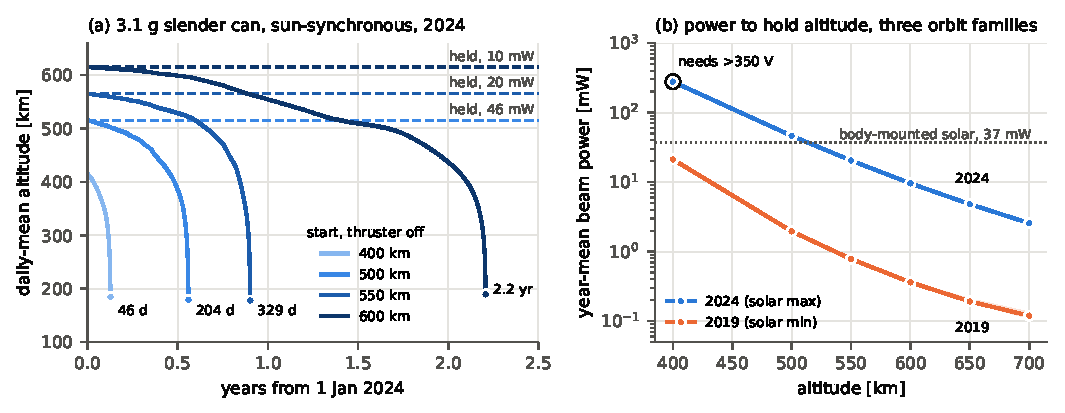
\includegraphics[width=0.9\linewidth]{missions.pdf}
  \begin{itemize}\small
    \item Year-long propagations, real F10.7/Ap, per-5-min plasma + drag;
          the servo picks $(V, I)$ each step.
    \item \textbf{Closes on skin-harvested power at 550--600\,km}; impulse-%
          closes (power-bound) at 500\,km; \textbf{does not close at 400\,km}
          for this body.
    \item Slender bodies (drag buys silhouette, collection buys skin) reopen
          400\,km -- geometry run planned.
  \end{itemize}
\end{frame}

% 11 --------------------------------------------------------------------------
\begin{frame}{How we know: the evidence stack}
  \begin{columns}
    \column{0.5\textwidth}
      \small\textbf{Per run (all gated):}
      \begin{itemize}\small
        \item Frozen, hashed physics config; manifest with seed, code
              version, git commit; interrupted runs discarded, never resumed.
        \item 7--8 acceptance gates fixed \emph{before} the run; zero waived.
        \item Ledger vs.\ independent particle dumps: agreement at
              $10^{-9}$ (gate $2\times10^{-2}$).
      \end{itemize}
    \column{0.48\textwidth}
      \small\textbf{Campaign-level:}
      \begin{itemize}\small
        \item Validation ladder below every thruster stage: thermal
              collection $\pm$1\% vs theory $\to$ biased $\to$ floating
              $\to$ gun rungs.
        \item Code-to-code parity (migrated vs predecessor implementation):
              $\varphi$ 0.05\%, escape 0.001\%, $F$ 0.09\%.
        \item Convergence: PPC$\times$2 shifts every metric $\le$0.05\%;
              $dt$, seed $\le$0.5\% (predecessor); grid
              ($0.15\to0.10$\,mm): $F$ $+4.0$\%, KE $+7.4$\% -- carried as
              the error band, sign conservative for all gates.
      \end{itemize}
  \end{columns}
\end{frame}

% 12 --------------------------------------------------------------------------
\begin{frame}{Where the model is blind --- and the two runs that fix it}
  \begin{itemize}\small
    \item \textbf{Density axis}: all runs at one dayside row; the night-side
          corridor edge (thin, cold plasma $\to$ float toward 50\,V) is
          flagged extrapolation. $\to$ \emph{night-row run.}
    \item \textbf{Geometry axis}: collection exponent is provably
          shape-dependent (sphere 1, cylinder 0.5; can measured 0.82--0.89).
          $\to$ \emph{slender-body run (planned), pre-registered
          hypotheses $\varphi \approx 4$--5\,V vs tens of V.}
    \item Reduced ion mass ($400\,m_e$ vs O$^+$ 29\,166); stationary plasma
          (no ram wake); RZ symmetry, no geomagnetic field; powers are beam
          power $I\,V$ (converter/cathode overheads not included).
  \end{itemize}
  \vspace{1ex}
  \small Every mission row outside the measured envelope is counted and
  flagged, never averaged in -- the flagged bucket \emph{is} the future-work
  list.
\end{frame}

% 13 --------------------------------------------------------------------------
\begin{frame}{``Why not a tether?''}
  \begin{itemize}\small
    \item Conceded: per watt, electrodynamic-tether thrust at km scale beats
          any reaction engine, including this one.
    \item At gram scale the comparison inverts:
    \begin{itemize}\small
      \item a 5\,mm vehicle vs.\ a deployed, stabilized conductor
            $10^4$--$10^6\times$ its own length (libration control,
            meteoroid survivability);
      \item thrust constrained to the $I\mathbf{L}\times\mathbf{B}$
            direction;
      \item and a \emph{bare} tether still needs electron collection and
            emission at its ends -- \textbf{the same contactor physics this
            device is, minus the tether}.
    \end{itemize}
    \item Related flown physics is our foundation, not our competitor:
          bare-tether OML collection (Sanmart\'in 1993), PMG plasma
          contactors (1993), E-sail electron gun (Janhunen).
  \end{itemize}
\end{frame}

% 14 --------------------------------------------------------------------------
\begin{frame}{Take-away}
  \begin{enumerate}
    \item \textbf{The frontier is measured}: 3.4\,nN @ 12\,mW to 30\,nN @
          189\,mW, $F/P \propto 1/\sqrt{V}$, all gates PASS, predictions
          pre-registered.
    \item \textbf{The thrust is real}: full-return null closes to zero;
          return-channel momentum gated at 1--9\% of beam thrust.
    \item \textbf{The mission corridor is honest}: closes at 550--600\,km on
          the spacecraft's own skin; fails at 400\,km and says so.
  \end{enumerate}
  \vspace{2ex}
  \centering
  \large\emph{Cheap to test on orbit: it's a gun and a hole.}\\[1ex]
  \normalsize A propellantless thruster whose optimal controller is a
  two-line servo on its own floating potential.
\end{frame}

% ============================ BACKUPS ========================================
\appendix
\begin{frame}{Backup: the U-valley and the no-equilibrium boundary}
  \begin{itemize}\small
    \item Predecessor campaign, five converged runs at fixed 13.6\,nN
          (78--300\,V): specific power $P/F$ = 5.18 / 4.44 / \textbf{4.31} /
          5.02 / 5.90\,mW/nN -- a shallow U.
    \item Below $\sim$91\,V at that demand: \textbf{no equilibrium at all}
          (space charge blows the beam open; the can eats its own beam) --
          confirmed by a pre-registered counterexample run.
    \item Left arm taxes: charging ($\varphi/V$: 27.6\% at 78\,V vs 8.7\% at
          200\,V) and escape collapse (68.6\% at 78\,V).
    \item Hence the rule: \emph{sit at the valley for the instantaneous
          demand -- never as low as feasible.}
  \end{itemize}
\end{frame}

\begin{frame}{Backup: settle time and the 300\,V late-slope caveat}
  \begin{itemize}\small
    \item Body $\approx$ capacitor charged by the escaping beam:
          $\tau \approx C\varphi/I_{\mathrm{esc}} \approx 28$\,ns at the
          reference; every run spans $\approx$29$\tau$.
    \item At high $\chi$ the sheath equilibrates on the \emph{ion}
          timescale: the 300\,V late slope decayed $+44 \to +27$\,mV/ns but
          was nonzero at 800\,ns.
    \item Settled-value extrapolation: $\varphi_\infty \approx 42$--48\,V --
          inside the 50\,V gate, carried through the $\alpha$ fit as the
          0.85--0.89 band.
    \item The caveat was pre-registered \emph{with} the hypothesis test.
  \end{itemize}
\end{frame}

\begin{frame}{Backup: numerics detail}
  \begin{itemize}\small
    \item WarpX 26.5 (GPU), RZ electrostatic, embedded-boundary conductor
          with per-step charge-pump float update; particle reservoir
          (infinite-ionosphere recycle).
    \item Grid 0.15\,mm ($\lambda_D = 1.97$\,mm); CFL $dt$; 16 ppc;
          800\,ns per production run; $\sim$7\,h on an RTX 3060.
    \item PPC$\times$2 at the anchor: $F$ +0.05\%, $\varphi$ +0.04\%,
          escape $-0.00$\%, KE $-0.01$\% (all 8 gates PASS). Grid
          $0.15\to0.10$\,mm (matched 536\,ns window): $F$ $+4.0$\%,
          $\varphi$ $-1.8$\%, KE $+7.4$\%.
    \item Reduced ion mass $400\,m_e$: ladder-wide, disclosed; float
          sensitivity to ion mass not yet measured.
  \end{itemize}
\end{frame}

\begin{frame}{Backup: slender-body hypotheses (run planned)}
  \begin{itemize}\small
    \item Drag buys the ram silhouette; collection and solar power buy the
          skin. \O10$\times$100\,mm rod: chipsat drag, 10$\times$ skin,
          100--200\,mW harvest, tens of grams.
    \item Pre-registered discrimination at the 200\,V anchor demand
          (\O10$\times$30\,mm, 3.24$\times$ area):
          \textbf{A} -- area-only scaling, $\varphi \approx 4$--5\,V;
          \textbf{B} -- cylinder-limit lateral collection, $\varphi$ tens of
          volts (possible benign-gate failure = design-critical finding).
    \item Thin-radius limit connects to flown bare-tether collection
          physics.
  \end{itemize}
\end{frame}

\begin{frame}{Backup: propellant accounting}
  \begin{itemize}\small
    \item ``Propellant'' = ambient electrons: $\dot m = (m_e/e)\,I \approx
          2\times10^{-15}$\,kg/s at 0.342\,mA $\approx$ \textbf{60\,ng/year}.
    \item Effective $I_{\mathrm{sp}} \sim 10^{6}$\,s -- not a merit figure
          (electrons are nearly free momentum-poor mass), quoted only for
          the EP bookkeeping.
    \item Five years of nN thrust $\approx$ 5\,N\,s $\approx$ 0.3\,g of
          electrospray propellant: the argument for this device is never
          propellant \emph{mass} -- it is the \textbf{dry-system floor}
          (tank+feed+valves+PPU $\approx$ 0.3--1\,kg does not shrink to
          gram scale).
  \end{itemize}
\end{frame}

\end{document}
